
\documentclass{article}
\usepackage[T1]{fontenc}
\usepackage[right=1cm, left=1cm, top=1cm, bottom=2cm]{geometry}
\usepackage{parskip}
\usepackage{circuitikz}

\usepackage{listings}
\usepackage{mathtools}
\usepackage{relsize}
\usepackage{graphicx}
\usepackage{float}
\usepackage{pgfplots}\pgfplotsset{compat = 1.18}

\title{Software Enginnering Fall 2023-2024 \\ VALUNI Proposal}
\author{  
Hussein Heggi 	\and
Ahmed Waseem Raslan 	\and
Sarah Elsamanody 	\and
Nour Abdalla 	\and
Youssef Elmahdy	\and
Ahmed Elbarbary	\and 
Ahmed Jaheen}
\usepackage{titling}
\renewcommand\maketitlehooka{\null\mbox{}\vfill}
\renewcommand\maketitlehookd{\vfill\null}  

\begin{document}

\begin{titlingpage}
\maketitle
\end{titlingpage}

\break

\tableofcontents

\break

\section{Project Description}
\quad VALUNI is a platform where students have the opportunity to share their experiences and exchange knowledge and feedback regarding both professors and courses.  It would play a vital role in helping students hold sufficient knowledge that could ease up the process of choosing classes and preparing for exams. Our objective is to create a safe, dependable and organized environment that allows students to express their opinions in an honest and respectful way. We aim to motivate students when rating or writing their reviews through anonymity, and at the same time having certain guidelines that must be followed when using VALUNI. This will not only assist students, but also the overall University community including diverse facilities and professors. 

\section{Usage}
$\bullet$ Search for professors and courses feedback.  

$\bullet$ Rate professors on a variety of criteria which are explanation, fairness, organization, leniency, and accessibility.

$\bullet$ Rate courses based on difficulty level, workload, and learning outcomes.

$\bullet$ Course Evaluations per semester for universities to measure the educational quality.

\section{Risks} 

\subsection{Community Risks}
$\bullet$ \textbf{Defamation:} Students may post false or misleading reviews of professors, which could damage the professor's reputation and career.

$\bullet$ \textbf{Bias:} Student ratings of professors may be biased. For example, distinct students may go through different experiences such as receiving undesired grades , influencing the integrity of their ratings.

$\bullet$ \textbf{Increased Reliance on student feedback:} Professors may rely too heavily on student feedback for validation, which could negatively impact their teaching style. In addition, students may depend on the review itself without actually giving the professor a chance.

\subsection{Development Risks} 

$\bullet$ The website is not liked by its main target audience as well as not being used by the student body which will defeat the whole purpose of the website.

$\bullet$ The website is not perfectly secured which can lead to privacy issues and data breaches.

$\bullet$ The cost of developing and maintaining the website could be high which could result in problems with financial sustainability.

$\bullet$ The website may not be well-received by professors which can make the website unsuccessful.



\section{Motivation} 

\quad Nowadays, the majority of students find it difficult to navigate the right path when it comes to making decisions during their registration periods. It is a well known hustle amongst students as continuously trying  to find the suitable courses and professors that fits their best interest is a challenge.  In fact, some students initiated solving this problem by creating  RateAUCProfessors, a FaceBook group, to provide reviews about Professors and pass on evaluations to next colleagues. Eventually, some of the group members started posting content that is out of context which made it lose its academic focus. Not to mention, the data keeps increasing each semester which makes it difficult for students to search in an efficient way. Therefore, we came up with VALUNI  where our main purpose is to constantly and effectively serve the educational community. This is because it would incorporate not only accessible reviews on courses and professors but also help collect evaluations at the end of each semester; aiding the university to adopt rightful and recent evaluations regarding each aspect of the overall educational level. 

\break
\section{Product Backlog}

\subsection{Functional Requirements}

	\quad User authentication 
	\vspace{-0.2cm}

	\qquad \scriptsize User login and verification that user is a university student \normalsize

	\quad Rating Courses

	\quad Rating Professors

	\quad Writing out a review with Rating
	\vspace{-0.2cm}

	\qquad \scriptsize When Reviewing students have the option to write a review with the parameterized rating \normalsize

	\quad Parameterized Rating
	\vspace{-0.2cm}

	\qquad \scriptsize Students can rate professors and courses on different parameters, such as workload, leniency \normalsize

	\quad Filtered Search on parameters 
	\vspace{-0.2cm}

	\qquad \scriptsize Students can filter out result or search for courses and professors based on parameters \normalsize

	\quad Reporting reviews 

	\quad Moderaters remove reviews

	\quad Editing Reviews

	\quad Admin ( university ) access to review data 
	\vspace{-0.2cm} 

	\qquad \scriptsize University can access critical semster review analytics as well as overall analytics \normalsize

	\quad Search for courses 

	\quad Search for professors 



\subsection{Non Functional Requirements} 

	\quad Fluid, Simple UI

	\quad Secure

	\quad Auto removing profanity on reviews

	\quad Prevent Review Bombing

	\quad Reviewer Anonymity

	\quad Customer Service ( for universities )

	\quad Performance

	\quad Scalability

\section{Use Case Diagram} 

\begin{center}
	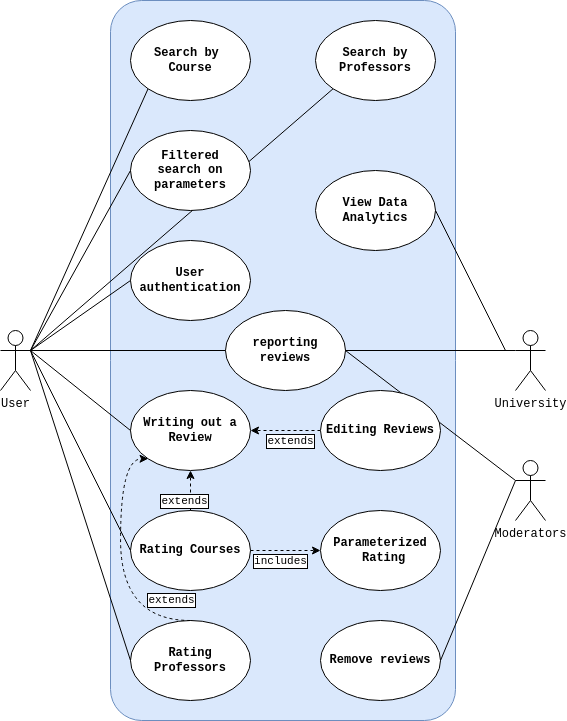
\includegraphics[scale=0.5]{../requirements_specification/USECASE.drawio.png}	
\end{center}

\section{MVP Requirements}

	\quad User authentication (login etc)

	\quad User data encryption

	\quad Rating Courses

	\quad Rating Professors

	\quad Writing out a review with Rating

	\quad Parameterized Rating

	\quad Filtered Search on parameters	

	\quad Editing Reviews


\section{High Level Design Architecture}

\begin{center} 
	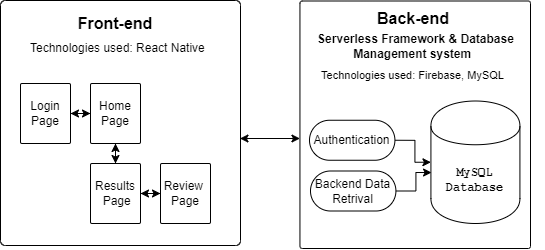
\includegraphics[scale=0.5]{./projectUml.drawio.png}
\end{center}

\quad We will be using a serverless framework with firebase for the website. Validating users will be done through access to university's database. The MVP however will work on mock-up data since gaining access to university's data during development is unrealistic.

\section{Conclusion}

\quad Deriving new alternatives ensures the continuous improvement of educational systems to ease up difficulties presented by choosing courses or professors. We will achieve this by implementing standard moderation procedures and easiness in frontend navigation. Additionally,  VALUNI is a new platform that integrates RateAUCProfessors on a higher technological and beneficial level; however, it comes with new risks that need to be tackled to ensure the integrity and privacy of its users. 




\end{document}


